
% if you need a4paper uncomment this line
%\documentclass[a4paper, 12pt, conference]{ieeeconf}   

\documentclass[a4paper, 12pt, journal, onecolumn]{IEEEtran}
\usepackage{geometry}
\newgeometry{tmargin=3cm, bmargin=3cm, lmargin=3.5cm, rmargin=3.5cm}

\IEEEoverridecommandlockouts                       
%\overrideIEEEmargins
% See the \addtolength command later in the file to balance the column lengths
% on the last page of the document



% The following packages can be found on http:\\www.ctan.org
%\usepackage{graphics} % for pdf, bitmapped graphics files
%\usepackage{epsfig} % for postscript graphics files
%\usepackage{mathptmx} % assumes new font selection scheme installed
%\usepackage{times} % assumes new font selection scheme installed
%\usepackage{amsmath} % assumes amsmath package installed
%\usepackage{amssymb}  % assumes amsmath package installed

\title{\LARGE \bf
Report on Saluki: Finding Taint-style Vulnerabilities with Static Property Checking
}
\author{Jacek Janczura \\ \small{404975, Software Engineering of Embedded Systems, Technische Universität Berlin, {\tt janczura.jacek@gmail.com}}}%

\usepackage{graphicx} %package to manage images
\graphicspath{ {images/} }
%\usepackage{caption} % it throws the warning
\usepackage[style=base]{caption}
\usepackage{enumitem}

\usepackage[]{siunitx}
\usepackage{textcomp}

\usepackage{listings}
\usepackage{fancyhdr}
\fancyhf{}
\rhead{Jacek Janczura}
\lhead{Report on Saluki: Finding Taint-style Vulnerabilities }
\rfoot{Page \thepage}
\setlength{\headheight}{14pt}


\usepackage{xcolor}
\DeclareCaptionFont{white}{\color{white}}
\DeclareCaptionFormat{listing}{%
  \parbox{\textwidth}{\colorbox{gray}{\parbox{\textwidth}{#1#2#3}}\vskip-4pt}}
\captionsetup[lstlisting]{format=listing,labelfont=white,textfont=white}
\lstset{frame=lrb,xleftmargin=\fboxsep,xrightmargin=-\fboxsep}

\begin{document}

\maketitle
\thispagestyle{fancy}
\pagestyle{fancy}


%%%%%%%%%%%%%%%%%%%%%%%%%%%%%%%%%%%%%%%%%%%%%%%%%%%%%%%%%%%%%%%%%%%%%%%%%%%%%%%%
\begin{abstract}
\textbf{This report explains the architecture and Saluki's idea for checking taint-style (data dependent) security properties in a binary code. Saluki is a new tool which is capable of finding a large number of CWS\footnote{CWS- Common Weakness Enumeration - list of software weakness types \cite{a2}} vulnerabilities in real programs. Saluki uses a mixture of static and dynamic taint analysis to follow data dependent facts. Saluki is proved to be capable of finding vulnerabilities in COTS\footnote{ COTS - Commercial off-the-shelf -  products are packaged solutions which are then adapted to satisfy the needs of the purchasing organization \cite{a1}} including 0-days.}

\end{abstract}


%%%%%%%%%%%%%%%%%%%%%%%%%%%%%%%%%%%%%%%%%%%%%%%%%%%%%%%%%%%%%%%%%%%%%%%%%%%%%%%%
\section{INTRODUCTION}

Recently vendors continue to ship vulnerable programs. Unfortunately to protect their "know how" and intellectual property, source code is not shipped. That is a big issue because analysis of binaries is far more complicated. To protect the privacy and security of the users and to analyse/check the binaries shipped by the vendors, some new tools and techniques for finding vulnerabilities in COTS need to be introduced. \cite{saluki} 

\section{Theoretical introduction}

To understand steps of execution and Saluki's internal architecture following introduction needs to be done.

\subsection{Control Flow Graph - CFG}

Representation, using graph notation, of all paths that might be traversed through a program during its execution including all the jumps, all the reads from the registers is called Control Flow Graph (Fig. \ref{fig:CFG}). CFG shows all of the possible states of the program execution and the possible paths to achieve that state.


\begin{figure}[ht]
    \centering
    \captionsetup{justification=centering}
    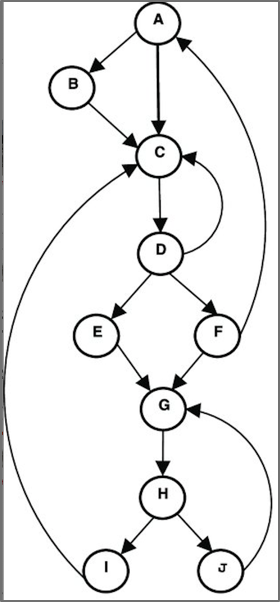
\includegraphics[width=0.25\textwidth]{CFG.png}
    \caption{Sample Control Flow Graph \cite{a3} }
    \label{fig:CFG}
\end{figure}


\subsection{Approximation}

In Fig. \ref{fig:approximation} set of all possible states that can be achieved by the program during its execution is assigned with letter A. To cover that state all the possible inputs needs to be supplied to the program which will result in all of the possible states in the output. Unfortunately supplying all of the possible inputs is not possible which is the reason for using the approximation.

\subsection{Under Approximation}

Under approximation means that we supply only the part of the possible states during the execution of the program. In that case we can not cover all of the possible inputs but only the subset of it. It results in the subset of all the possible outputs. Under approximation in Fig. \ref{fig:approximation} is assigned with UA and is a subset of A. \cite{a4}

\subsection{Over Approximation}

Over approximation in case of achieving the CFG states, means that the set of the states in over approximation is bigger than the set of the all possible states that can be achieved by the program in CFB. Over approximation in Fig. \ref{fig:approximation} is assigned with OA and A is a subset of OA. \cite{a4}

\begin{figure}[ht]
    \centering
    \captionsetup{justification=centering}
    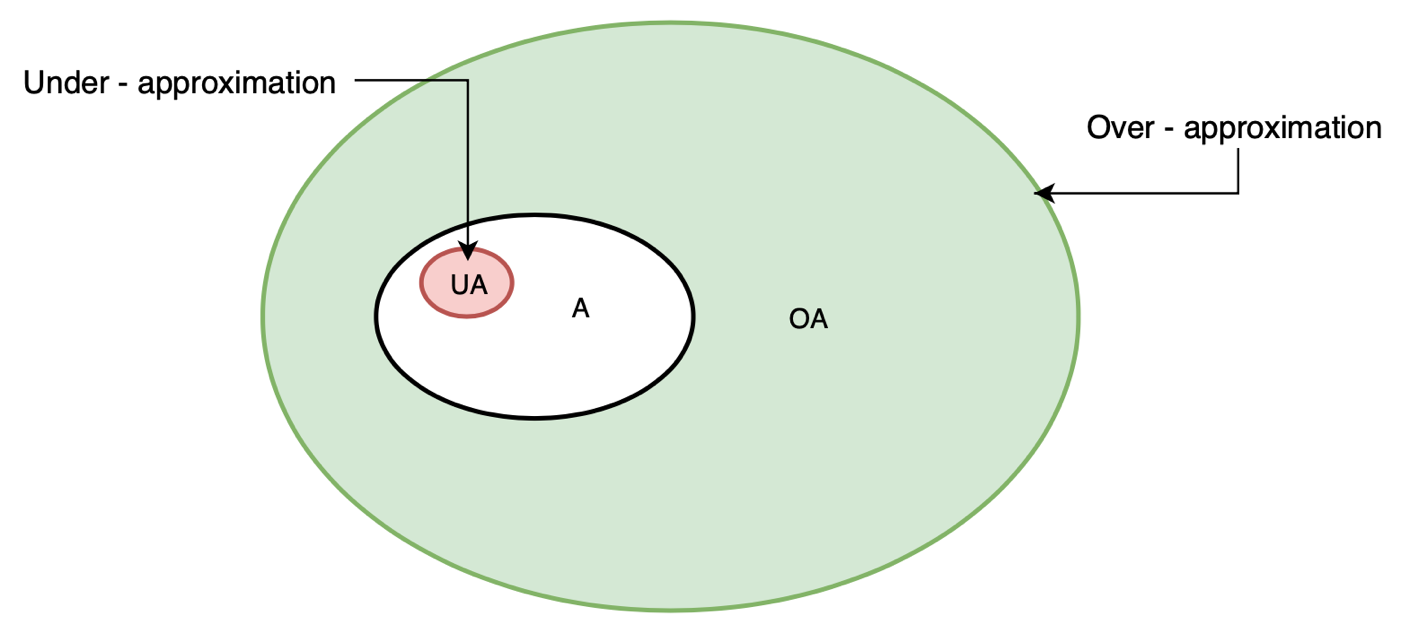
\includegraphics[width=0.8\textwidth]{approximation.png}
    \caption{Visualisation of over and under approximation \cite{a3} }
    \label{fig:approximation}
\end{figure}

\subsection{Mixed Approximation}

Mixed approximation is a subset of the states that are reachable by the program and the states that are not possible to be reached in CFG.   

\section{Taint-style Vulnerabilities}

The term taint-style vulnerabilities has its roots in taint analysis, a technique for tracing the propagation of data through a program. One goal of taint analysis is to identify data flows from attacker-controlled sources to security-sensitive sinks that do not undergo sanitization.\cite{a5} \cite{a6}

Taint analysis can be used for example to check if the data received to a socket by the function $receive()$ and saved in some buffer does not leak. It means that it is not sent away by the function $send()$.

In an example shown in a Fig. \ref{fig:taint} functions and buffers that cannot be dependent one to another need to be specified. Data saved by $receive(*buf_a)$ can not be send away by $send(*buf_b)$. 
\\

Taint analysis is divided into three steps:\\
\begin{itemize}
\item \textbf{Seeding} - during seeding all the $receive()$ functions need to be find in the CFG. Than the memory cells where the received data is saved need to be tainted. Each tainted memory cell has its index number for tracing the leakage path and taint flag. Taint flag informs if that specify memorycell has been already tainted or not.\\
\item \textbf{Propagation} - taint propagation resemble spreading of a virus. In propagation step all the paths in CFG from $receive(*buf_a)$ to $send(*buf_b)$are traversed and each memory cell is tainted.\\
\item \textbf{Checking} - during checking each one of the memory cells in $buf_b$ is checked for the taint. Presence of the taint in $buf_b$ means that received data may be leaked away\\
\end{itemize}

\begin{figure}[ht]
    \centering
    \captionsetup{justification=centering}
    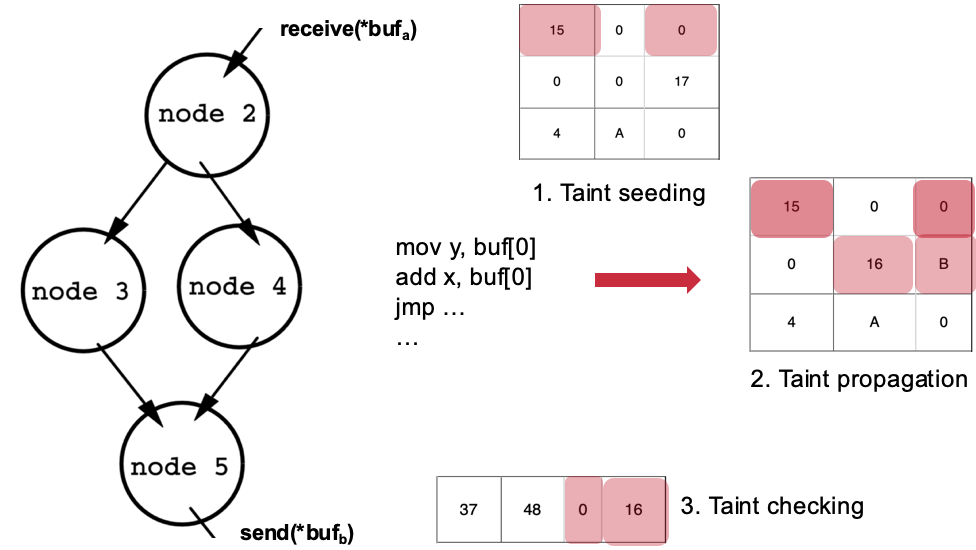
\includegraphics[width=0.9\textwidth]{Taint.png}
    \caption{Visualisation of taint analysis}
    \label{fig:taint}
\end{figure}

\subsection{Dynamic taint-style analysis}

Dynamic taint-style analysis is the analysis done during the run time. Program is run and a few possible inputs are supplied. After that, tainted data triggered by the program at the run time, is followed. Dynamic taint-style analysis is an example of under approximation because all of the states are reached during the runtime of the program - are part of CFG. \cite{a6}\cite{a7}

\begin{itemize}
\item Pros:	

\begin{itemize}
\item It is fast	
\item No false positive
\end{itemize}

\item Cons:

\begin{itemize}
\item Detect only bugs triggered by an executed path at the run time
\item Always starts at the entry point
\end{itemize}

\end{itemize}

\subsection{Static taint-style analysis}

Static taint-style analysis is an example of over approximation. Static analysis in contrary to the dynamic is not done during the run time. Due to the large number of an external unreachable by the program in the run time states in the static analysis we observe a large number o false positives. On the other hand all the states reachable by the program are the subset of the states reached by static analysis. It means that among many false positives, all of the possible bugs will be caught. \cite{a5}\cite{a6}

\begin{itemize}
\item Pros:	

\begin{itemize}
\item Detects all of the bugs

\end{itemize}

\item Cons:

\begin{itemize}
\item Many false positives

\item Takes a long time
\end{itemize}

\end{itemize}

\section{Saluki Architecture}

In contrary to a static and a dynamic taint-analysis Saluki creators came up with a new and novel approach. Instead of under approximating the states in a run time or statically slowly over approximating all the possible and and impossible states, in case of Saluki random parts of code are executed. 

In a seeding part all instructions and policies that a user wants to check are being found in a control flow graph and tainted. Than in a propagation part, plugin called $\mu$flux executes random parts of the CFG supplying the random input and goes down the graph. 

Saluki does not need to start every time from the beginning. Additionally randomisation of an execution point, lets Saluki go deeper into the CFG than during a normal dynamic analysis. On the other hand randomisation of the input makes Saluki to achieve a normally unreachable states like in over approximation. That is why the states approximation of Saluki is the mixed one.
\\

Saluki's execution can be divided into five steps.
Its overall architecture is shown in a Fig. \ref{fig:saluki}.  \cite{saluki} :

\begin{enumerate}[label=\Alph*]
\item Load in the specification.
\item Parse the binary into an intermediate representation (IR\footnote{Creating IR can be simplified for better understanding to creating a control flow graph of whole binary}) suitable for analysis. 
\item Run $\mu$flux\footnote{$\mu$flux works as a taint propagation} to collect data flow facts about executions from every specified source.
\item Run a solver over the policies, program, and collected facts. The solver determines whether the property holds or not.
\item Saluki outputs example paths where the property does not hold. The actual output is not a full path, but instead a condensed form of the tainted instructions and a flow ID.
\end{enumerate}

\begin{figure}[ht]
    \centering
    \captionsetup{justification=centering}
    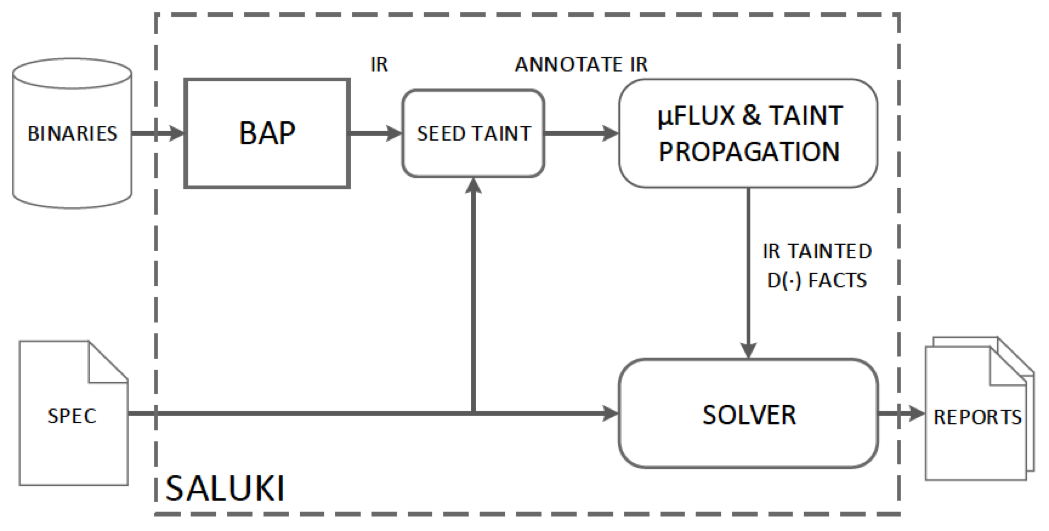
\includegraphics[width=0.85\textwidth]{saluki.png}
    \caption{Saluki Architecture \cite{saluki}}
    \label{fig:saluki}
\end{figure}

\textit{Specification: } The first step of running the Saluki is loading the vulnerabilities specification. Saluki has already implemented a database - CWE\footnote{CWE - community-developed list of common software security weaknesses} with dozens of vulnerabilities. Additionally user can load customised, user-defined policies using the Saluki's language.\\

%\belowcaptionskip=-10pt

\begin{lstlisting}[label=saluki-code,caption=Command injection example]
    prop recv_to_system ::=
    recv(_,*buf,_,_), system(*cmd) |- never
    s.t. cmd/buf
\end{lstlisting}

In the Listing 1, there is shown a policy in Saluki language for finding a command injection. 

Command injection vulnerabilities arise when input flows from an input source to a sink function that executes code. 

In this case system should never use data from recv (data received from the socket). Otherwise we can assume that a command in a system shell was executed - system used data from the socket. 

The only limitation is that Saluki does not specifically reason about memory corruption vulnerabilities such as buffer overflows.

\bigskip

\textit{Binary processing:} The binary is loaded to the Saluki. Than Saluki runs a BAP\footnote{BAP - BinaryAnalysisPlatform - https://github.com/BinaryAnalysisPlatform/} (BinaryAnalysisPlatform) an open-source plugin-based binary analysis framework. BAP converts binary code into control flow graph - intermediate representation.\cite{a8} 
\bigskip

\textit{Taint Seeding:} Saluki analyzes the specification for variables used in constraints. Each constraint variable is linked to
a program location, which is then marked in the IR as a taint
seed. In our running example, cmd is a constraint variable used
in recv, causing Saluki to identify the proper memory location
corresponding to the cmd argument in all terms named recv.
As is customary, Saluki uses unique identifiers to identify each
taint seed.\cite{saluki}
\bigskip

\textit{$\mu$flux:} $\mu$flux is implemented as a custom interpreter that runs random parts of CFG and propagates the taint across the memory. $\mu$flux start taint propagation from the instructions picked from specification and marked during the seeding. Than it executes parts of CFG randomly. $\mu$flux explore the paths regardless of the branch predicate and ignore context of data.
\medskip

$\mu$flux stops execution when:
\begin{itemize}
\item Pre-defined max. instructions number was excited
\item Saluki call dynamically linked external function
\item Saluki hits a jump with an indirect target
\end{itemize}

\bigskip
\textit{The Saluki Solver:} In this step Saluki starts to follow the taint and tries to prove all properties specified in a policy. Saluki is constructive: it does not just say there is a violation, but gives the specific path and data dependencies used to show the property can be violated 



\section{Results and tests}

Saluki research group tested Saluki on many binaries and try to check it performance. They found two binaries where srand seed was time dependent, 6 new zero-days bugs in 5 COTS products, what is more they have found using Saluki Heartbleed in OpenSSL. Unfortunately in the same library Saluki showed 4 false positive alerts.
In Lighthttp Saluki research tteam found sommand injection to system, buffer overflow due to wrong usage of strcpy. Apart from OpenSSL and Lighthttp they found 3 SQL injections in some COTOS products and many more.


This experiments shows that Saluki may be useful but user needs to be aware that a false-positives may occur and check every alert. 


\section{Conclusions}

Saluki is not sound nor complete. The main advantage of it is that in comparison to other tools used to find vulnerabilities it’s fast. Unfortunately the authors of Saluki did not benchmark it against other tools which I think is a big drawback of the paper.

%%%%%%%%%%%%%%%%%%%%%%%%%%%%%%%%%%%%%%%%%%%%%%%%%%%%%%

\bibliographystyle{unsrt}
\bibliography{sample}

\end{document}
